\thispagestyle{plain}

\chapter*{Margaret Mead}
\addcontentsline{toc}{part}{Margaret Mead}

\begin{center}
	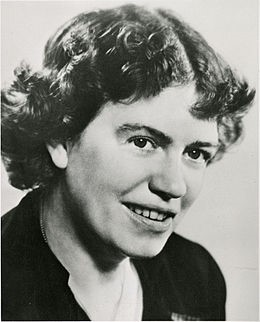
\includegraphics[scale=7]{MMead.jpg}
\end{center}

\paragraph{} Margaret MEAD est née le 16 décembre 1901 à Philadelphie d'un
professeur d'économie et d'une enseignante. Elle débute ses études à
l'université Pauw qu'elle quitte au bout d'un an pour étudier la psychologie à
l'université Barnard. Elle entre en 1923 dans le département anthropologique de
l'université Columbia. Elle obtient son doctorat en 1929 grâce à une thèse sur
la stabilité de la culture en Polynésie. Entre 1928 et 1935, elle fait de
nombreux voyages avec son troisième mari Reo Fortune. Elle donne naissance à sa
fille Mary Catherine Bateson Kassarjian qu'elle a eue avec son dernier mari
Gregory Bateson. Ses travaux portent notamment sur le rapport à la sexualité
dans les cultures traditionnelles de l'Océanie et du Sud-est asiatique. Elle a
notamment écrit ``le temps est venu, je crois, où nous devons reconnaître la
bisexualité comme une forme normale de comportement humain'' et ``un grand
nombre d'êtres humains - probablement la majorité - sont bisexuels en ce qui
concerne leur capacité à éprouver des sentiments amoureux''. Elle est morte des
suites d'un cancer le 15 novembre 1978. Elle a reçu la Médaille Présidentielle
de la Liberté à titre posthume en 1979. Elle est inscrite au National Women's
Hall of Fame.
